% This is LLNCS.DEM the demonstration file of
% the LaTeX macro package from Springer-Verlag
% for Lecture Notes in Computer Science,
% version 2.4 for LaTeX2e as of 16. April 2010
%
\documentclass{llncs}
%
\usepackage{makeidx}  % allows for indexgeneration
\usepackage[hidelinks]{hyperref}
\usepackage{graphicx}
\usepackage{listings}
\usepackage[utf8]{inputenc}
\usepackage[ngerman]{babel}

\hypersetup{
	pdftitle = {Objekt Algebra - Ein Lösungsansatz für das Expression Problem},
	pdfsubject = {Software-Development},
	pdfauthor = {Marco Buchholz, Max Golubew, Florian Winzek},
	pdfkeywords = {expression problem, visitor pattern, interpreter pattern, object algebra}, 
	colorlinks = false
}

%
\begin{document}
%
\frontmatter          % for the preliminaries
%
\pagestyle{headings}  % switches on printing of running heads
%
\mainmatter              % start of the contributions
%
\title{Objekt Algebra - Ein Lösungsansatz für das Expression Problem}
%
\titlerunning{Objekt Algebra - Ein Lösungsansatz für das Expression Problem}  % abbreviated title (for running head)
%                                     also used for the TOC unless
%                                     \toctitle is used
%
\author{Marco Buchholz%\inst{1}%\orcidID{0000-1111-2222-3333}
\and
Max Golubew%\inst{2}%\orcidID{1111-2222-3333-4444} 
\and
Florian Winzek%\orcidID{2222-3333-4444-5555}
}
%
\authorrunning{Marco Buchholz, Max Golubew, Florian Winzek} % abbreviated author list (for running head)
%
%%%% list of authors for the TOC (use if author list has to be modified)
\tocauthor{Marco Buchholz, Max Golubew, Florian Winzek}
%
\institute{Institute for Software Engineering and Programming Languages, Universität zu Lübeck\\
\email{marco.buchholz@student.uni-luebeck.de} \\
\email{max.golubew@student.uni-luebeck.de} \\
\email{f.winzek@student.uni-luebeck.de}}

\maketitle              % typeset the title of the contribution

\begin{abstract}
Das Expression Problem ist ein bekanntes Problem in der Funktionalen Programmierung. Hierbei geht es darum, dass ein Programm, welches aus Datenstrukturen und Funktionen besteht, in diese zwei Dimensionen weiterentwickelt werden soll, ohne das Programm neu kompilieren zu müssen. Die Komplexität des Programs darf ebenfalls nicht größer werden. In diesem Paper behandeln wir einen Ansatz, welcher das Problem lösen kann. In diesem Zusammenhang stellen wir das Konzept der Objekt Algebra vor. Wir werden Lineare Zeit Logik Formeln (LTL-Formeln) als anschauliches Beispiel benutzen. Um zu zeigen, dass die Objekt Algebra ein Programm auf einfache Art um Operationen und Datenstrukturen weiterentwickeln kann, werden wir zunächst eine Grundmenge von LTL-Formeln betrachten und diese dann um zusätzliche Formeln und Funktionen erweitern.

Der gesamte Sourcecode ist auf Github verfügbar\footnote{https://github.com/mbuchholz/ObjectAlgebra}.
\end{abstract}
%
\section{Einleitung} \label{sec:introduction}

Beim Expression Problem geht es speziell um Computerprogramme oder Algorithmen. Diese werden im Laufe der Entwicklung immer komplexer. Das bedeutet, es kommen neue Funktionen für bestehende Datentypen hinzu, aber auch neue Datentypen für aktuelle Funktionen. Diese beiden Dimensionen sollten beim Entwicklungsprozess möglichst dynamisch gehalten werden, damit das Programm nicht zu komplex wird. Oftmals muss der Code neu geschrieben und kompiliert werden. 
\cite{wadler98}

Es gibt einige Ansätze um zumindest einen der zwei Dimensionen dynamisch weiterzuentwickeln. Wir werden im folgenden Kapitel auf diese Ansätze eingehen und die Vor- und Nachteile erörtern. Im Anschluss stellen wir einen alternativen Ansatz vor, welcher beide Dimensionen gleichzeitig abdeckt. Zum Schluss zeigen wir eine mögliche Implementierung am Beispiel von LTL-Formeln.   

\section{Lösungsansätze} \label{sec:approaches}

In diesem Kapitel wollen wir zunächst ein wenig auf bekannte Software Pattern eingehen, die sich im Kern mit dem Expression Problem auseinandersetzen. Dies sind zum Einen das sogenannte \emph{Interpreter Pattern} und das \emph{Visitor Pattern}. Ein alternativer Ansatz stellt die sogennante \emph{Objekt Algebra} dar, auf welchen wir insbesondere eingehen werden. 

\subsection{Interpreter Pattern} \label{sec:interpreter}

Das \emph{Interpreter Pattern} ist eine Entwurfsmethode der Softwaretechnik und ermöglicht es Sätze einer Sprache auf Basis einer definierten Grammatik zu interpretieren. Vor allem bei wiederkehrenden Problemen, die oftmals ähnliche Lösungsansätze haben, wie z.B. das Auswerten von logischen Formeln, ist diese Technik sehr gut einsetzbar. Das Pattern besteht aus einer Abstrakten Klasse, welche eine Interpretationsfunktion bereistellt. Sämtliche Ausdrücke lassen sich in einer ableitenden konkreten Klasse einfach auswerten. Ein Satz kann nun also Schritt für Schritt in Unterausdrücke aufgeteilt werden, die dann ausgewertet werden. Es entsteht ein Syntaxbaum, der von einer Parserklasse aufgebaut wird. Anschließend wird die Interpretationsfunktion aufgerufen und der Baum wird ausgewertet. 

Da die Interpretation in den einzelnen Endknoten des Syntaxbaumes geschieht, ist es sehr einfach, das Programm um neue Knoten zu erweitern. Möchte man nun eine neue Operation hinzufügen, müsste man hingegen jeden einzelnen Knoten des Baumes um diese Funktionalität erweitern. Komplexe Grammatiken sind ebenfalls von Nachteil, da die Anzahl der benötigten Klassen schnell sehr hoch werden kann. Auch ein zu großer Syntaxbaum, kann zu Performanz Probleme führen. 
\cite{hills2011case}

\subsection{Visitor Pattern} \label{sec:visitor}
In der objektorientierten Programmierung bietet das Visitor Pattern die Möglichkeit, neue Operationen zu existierenden Objekten hinzuzufügen, ohne die Struktur zu modifizieren.

Mit dem Visitor Pattern werden zwei Klassenhierarchien definiert. Der \textit{Visitor} implementiert eine Operation, die an \textit{Elementen} (oder Datenvarianten) einer Objektstruktur ausgeführt werden kann. Dies ermöglicht es, neue Operationen unabhängig von den Klassen zu erstellen, indem neue Visitor hinzugefügt werden. \cite{GHJV94}

Das Klassendiagramm in Abbildung \ref{fig:visitor-pattern} zeigt ein Beispiel einer solchen Implementierung. Ein Element muss eine \textit{accept}-Methode implementieren, um einen Visitor zu akzeptieren. Diese Methode wird aufgerufen, wenn der Visitor eine Operation auf diesem Element ausführen will. Dabei wird als Argument eine Instanz des Visitors übergeben. In der \textit{accept}-Methode wird danach die \textit{visit}-Methode des jeweiligen Visitors für die eigene Instanz aufgerufen. Ein Visitor implementiert somit für jedes Element eine spezifische Operation.

Die beschriebene Logik der \textit{accept}- und \textit{visit}-Methoden ist ein \textit{double-dispatch} Machanismus und wird bei dem Visitor Pattern vorausgesetzt.

\begin{figure}[h]
	\centering
	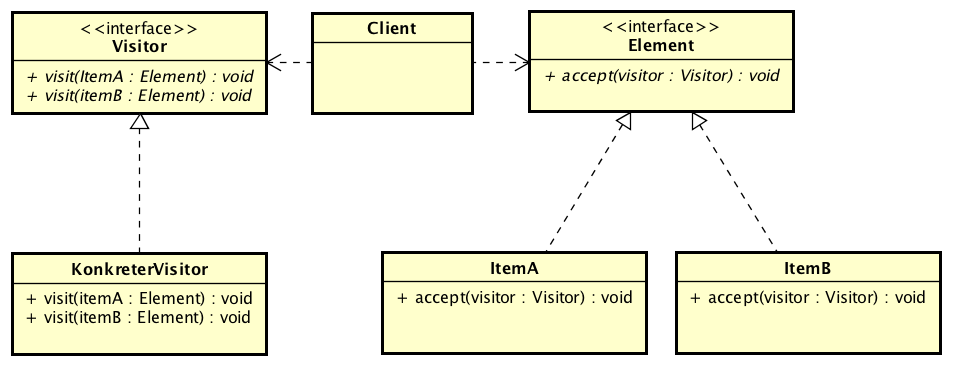
\includegraphics[width=\textwidth]{images/VisitorPattern.png}
	\caption{Beispiel Visitor Pattern}
	\label{fig:visitor-pattern}
\end{figure}

Nachfolgend werden die Vor- und Nachteile des Visitor Patterns zusammengefasst: \linebreak

\textbf{Vorteile:}
\begin{itemize}
	\item[$\bullet$] Mit dem Erstellen eines neuen Visitors, der das Visitor-Interface implementiert, können neue Operationen einfach hinzugefügt werden, ohne die Struktur zu modifizieren.
	\item[$\bullet$] Beim Hinzufügen einer neuen Operation erfolgt die Trennung der Logik durch einen neuen Visitor. Damit unterstützt das Pattern automatisch das \textit{Separation of Concerns} Prinzip.
\end{itemize}

\textbf{Nachteile:}
\begin{itemize}
	\item[$\bullet$] Werden in einer Element-Klasse Veränderungen vorgenommen, so muss wahrscheinlich auch die Visitor-Klasse überarbeitet werden.
	\item[$\bullet$] Beim Hinzufügen neuer Element-Klassen muss das Visitor-Interface mit den entsprechenden visit-Methoden erweitert werden.
	\item[$\bullet$] Das Visitor Pattern verletzt die Eigenschaft der Datenkapselung der Objektorientierten Programmierung. Die Schnittstelle der Elemente muss öffentliche Methoden beinhalten, damit der Visitor diese verwenden kann.
\end{itemize}

\subsection{Objekt Algebra} \label{sec:object-algebra}
Mit der Objekt Algebra wurde eine weitere Lösung für das Expression Problem vorgeschlagen \cite{Oliveira12}. Die Objekt Algebra basiert auf algebraischen Signaturen, die Werte einer abstrakten Menge zurück geben \cite{Guttag78}. Dabei wird eine generische Schnittstelle erstellt, deren Parameter vom abstrakten Typ sind. Eine solche Schnittstelle wird als \textit{Objektalgebra}-Schnittstelle bezeichnet.

\textit{Objektalgebra}-Schnittstellen  sind den \textit{Abstract-Factory}-Schnittstellen sehr ähnlich. Der Unterschied besteht darin, dass eine \textit{Factory}-Schnittstelle typischerweise eine bestimmte Klasse als Ergebnistyp verwendet, während die \textit{Objektalgebra}-Schnittstelle einen generischen Typ besitzt.

Die \textit{Factory}-Schnittstelle kann abgeleitet werden, indem der abstrakte Typ auf die spezifische Objektschnittstelle der zu erstellenden Objekte intsanziiert wird.

Objekt Algebra ist ähnlich zu dem Visitor Pattern. Während die Operationen bei dem Visitor Pattern in Visitor-Klassen implementiert werden und Datenvarianten als Elemente umgsetzt werden, verwendet die Objekt Algebra generische \textit{factory}-Schnittstellen um Datenvarianten zu repräsentieren. Die Operationen werden dann durch die Implementierung der factory umgesetzt.

Neue Datenvarianten können somit durch die Erweiterung der Schnittstelle hinzugefügt werden und die Operationen durch die Implementierung.


\section{Implementation} \label{sec:implementation}
In diesem Abschnitt geht es um eine konkrete Implementierung der in Abschnitt~\ref{sec:object-algebra} beschriebenen Objekt Algebra.
Dabei haben wir die \emph{Linear Temporal Logik (LTL)} \cite{pnueli77} verwendet, um die dort definierten Datentypen und Funktionen nachzubilden.
Genauer gesagt muss eine Datenstruktur für den \emph{abstract syntax tree (AST)} für LTL definiert werden.
Eine LTL-Formel ist durch die folgende Grammatik gezeigt:

\begin{lstlisting}
LTL ::= PROPOSITION | "!" LTL | LTL "||" LTL | LTL "&&" LTL
	| LTL "U" LTL | "X" LTL | "F" LTL
PROPOSITION ::= "TRUE" | "FALSE" | VARIABLE
VARIABLE ::= [a-z];
\end{lstlisting}\label{lst:grammar}

Daraus ergibt dich, dass der benötigte AST aus den Datenvarianten \emph{Disjunction}, \emph{Conjunction}, \emph{Unary}, \emph{Next}, \emph{Finally}, \emph{Negation}, \emph{Proposition} und \emph{Variable} besteht.
Um die Erweiterbarkeit der verwendeten Objekt Algebra zu zeigen, haben wir die Implementierung in drei evolutionäre Stufen aufgeteilt.
Zuerst gibt es nur die Operation \emph{Evaluation} zum Auswerten einer LTL-Formel auf einem gegebenen Wort. Außerdem ist die Datenvariante \emph{Finally} noch nicht implementiert.
Diese kommt dann in der zweiten Evolution dazu und in der letzten gibt es eine neue Operation mit dem Namen \emph{PrettyPrint}.
Diese liefert eine String-Repräsentation des AST, welche z.B. auf der dem Benutzer ausgegeben werden kann.

Anhand des Klassendiagramms in Abbildung~\ref{fig:object-algebra} zeigen wir die Implementierung der Objekt Algebra für LTL-Formeln.

\begin{figure}
	\centering
	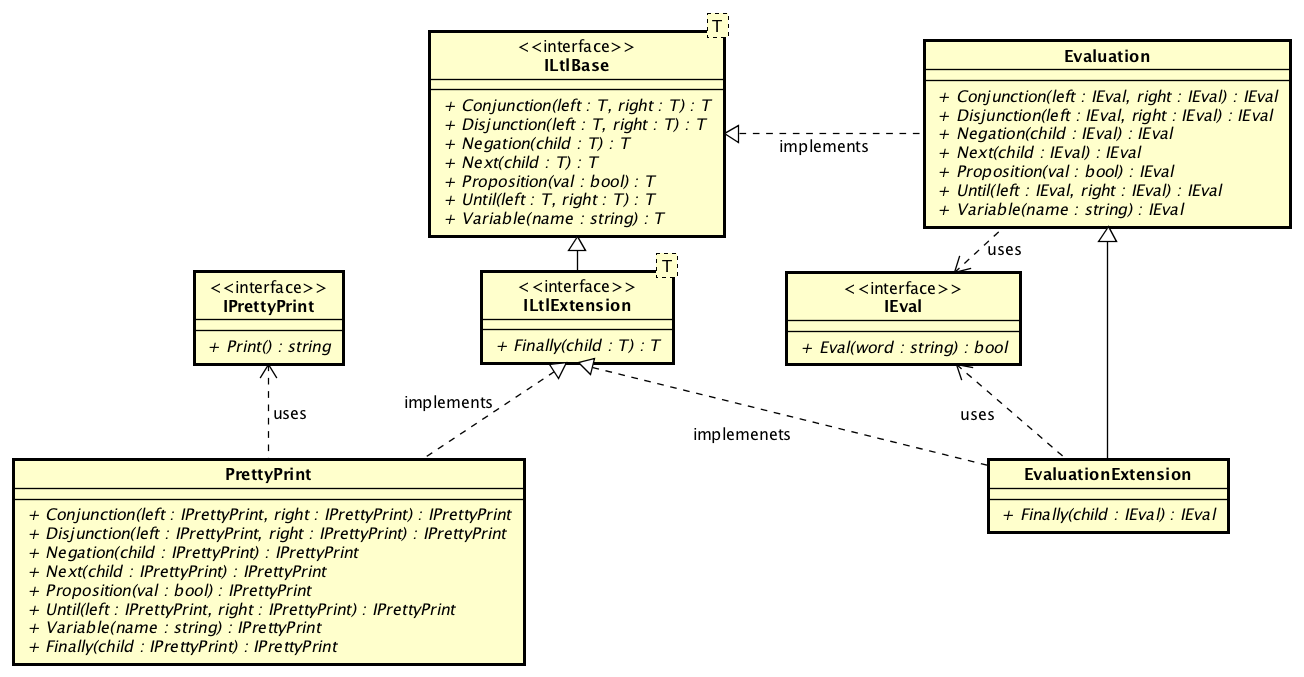
\includegraphics[width=\textwidth]{images/ObjectAlgebra.png}
	\caption{Ausschnitt des Klassendiagramms. Gezeigt sind die Klassen für die Objekt Algebra}
	\label{fig:object-algebra}
\end{figure}

\subsection{Evaluation - Evolution 1}
Die generische Schnittstelle \emph{ILtLBase} stellt das sogenannte \emph{Object Algerba Interface} dar (vgl. \cite[Abschnitt 3 S.6]{Oliveira12}).
Dieses bietet die Definitionen der Datenvarianten an, wobei darauf zu achten ist, dass es keine Methode für \emph{Finally} gibt.
Außerdem ist es durch die generische Typ-Definition unabhängig von einer Operation und trotzdem ist eine statische Typ-Sicherheit gegeben.
Die Klasse \emph{Evaluation} stellt nun die konkrete \emph{Objekt Algebra} dar.

Dafür wird die Schnittstelle \emph{ILtlBase} implementiert und dessen generischer Parameter an die Schnittstelle \emph{IEval} gebunden.
\emph{IEval} stellt unsere Operation dar und definiert daher die möglichen Methoden, die auf dem AST ausgeführt werden können.
Durch die Bindung des generischen Parameters auf die Operation wird nun von jeder Methode in \emph{Evaluation} eine konkrete Implementierung von \emph{IEval} zurückgeliefert.
Das bedeutet die Objekt Algebra arbeitet vergleichbar zu einer \emph{Factory}, da sie neue Typen des Interfaces (anonym) erstellt und zugleich dessen Instanzen erzeugt.

\subsection{Finally - Evolution 2}
Nun kommt die neue Datenvariante \emph{Finally} dazu. Dafür kann einfach eine neue Schnittelle erstellt werden, welche das vorhandene \emph{Object Algebra Interface} erweitert.
\emph{ILtlExtension} realisiert genau diese neue Schnittstelle. Dabei ist darauf zu achten,
dass auch diese ebenfalls generisch sein muss und ihren Template Parameter an die generalisierte Schnittstelle \emph{ILtlBase} übergibt und nicht durch eine konkrete Realisierung ersetzt.

Nun kann auch dafür eine \emph{Objekt Algebra} erstellt werden.
Dafür muss eine Klasse nur das neue \emph{Object Algebra Interface} implementieren. In unserer Implementation ist dies die Klasse \emph{EvaluationExtension}.
Um die Methoden aus der ersten Evolution nicht erneut implementieren zu müssen, wird \emph{Evaluation} erweitert.

\subsection{PrettyPrint - Evolution 3}
In der letzten Stufe wollen wir zeigen, wie eine neue Operation (\emph{PrettyPrint}) hinzugefügt werden kann. Dafür wird zuerst eine neue Schnittstelle \emph{IPrettyPrint} erstellt.
Jetzt wird nur noch eine entsprechende \emph{Object Algebra} benötigt. Die Klasse \emph{PrettyPrint} ist genau diese konkrete Realisierung.
Da sich in diesem Fall keine Datenvariante geändert hat, kann das vorhandene \emph{Object Algebra Interface} \emph{ILtlExtension} implementiert werden.
Die Klasse \emph{PrettyPrint} dient wieder als Factory und erzeugt somit Instanzen, welche unsere Schnittstelle \emph{IPrettyPrint} implementieren.
Das ist auch der Grund, warum \textbf{nicht} die Klasse \emph{EvaluationExtension} erweitert werden kann.

\section{Zusammenfassung} \label{sec:conclusion}

In diesem Paper haben wir uns mit dem Expression Problem befasst. Wir konnten zeigen, dass es Methoden und Pattern gibt, die sich dem Problem annehmen, aber nicht vollständig lösen konnten. Wir zeigten auch, dass das Interpreter und Visitor Pattern jeweils nur eine Dimension des Problems behandelt und motivierten aus diesem Grund einen alternativen Ansatz. Die Objekt Algebra ermöglicht es durch generische Schnittstellen neue Datentypen und neue Operationen der gegebenen Codebasis hinzuzufügen. Die Komplexität des Programmcodes ist dadurch nicht größer geworden. Anhand einer Beispielimplementierung haben wir den Sachverhalt noch einmal verdeutlicht. Die Objekt Algebra schafft es beide Dimensionen des Expression Problem zu behandeln und ist gleichzeitig eine elegante Programmiermethodik.


%
% ---- Bibliography ----
%
\begin{thebibliography}{5}
%

\bibitem{wadler98}
Wadler, P.:
The Expression Problem.
E-Mail Discussion (1998),
\url{http://homepages.inf.ed.ac.uk/wadler/papers/expression/expression.txt}

\bibitem{hills2011case}
Hills, Mark and Klint, Paul and Van Der Storm, Tijs and Vinju, Jurgen.
A case of visitor versus interpreter pattern.
International Conference on Modelling Techniques and Tools for Computer Performance Evaluation

\bibitem{Odersky05}
Odersky, M., Zenger, M.:
Independently Extensible Solutions to the Expression Problem. 
In FOOL'05

\bibitem{pnueli77}
Pnueli, A.:
The temporal logic of programs.
In 18th Annual Symposium on Foundations of Computer Science, Providence, Rhode Island, USA, 31 October - 1 November 1977, pages 46-57, IEEE Computer Society, 1977

\bibitem{GHJV94}
Gamma, E., Helm R., Johnson R. and Vlissides J.:
Design Patterns: Elements of Reusable Object-Oriented Software.
Addison-Wesley Professional Computing Series, Pearson Education, 1994

\bibitem{Parr09}
Parr, T.:
Language Implementation Patterns: Create Your Own Domain-Specific and General Programming Languages.
Pragmatic Bookshelf, 2009

\bibitem{Oliveira12}
Oliveira, B., Cook, W.:
Extensibility for the Masses - Practical Extensibility with Object Algebras.
In ECOOP 2012 -- Object-Oriented Programming: 26th European Conference, Beijing, China, June 11-16, 2012, pages 2-27, Springer Berlin Heidelberg

\bibitem{Guttag78}
Guttag, J., Horning, J.:
The algebraic specification of abstract data types.
In Acta Informatica Vol. 10, pages 27-52, March 1978

\end{thebibliography}
\end{document}
